% Options for packages loaded elsewhere
\PassOptionsToPackage{unicode}{hyperref}
\PassOptionsToPackage{hyphens}{url}
%
\documentclass[
]{book}
\title{Rethinking Companion}
\author{Wade VanderWright}
\date{2022-05-18}

\usepackage{amsmath,amssymb}
\usepackage{lmodern}
\usepackage{iftex}
\ifPDFTeX
  \usepackage[T1]{fontenc}
  \usepackage[utf8]{inputenc}
  \usepackage{textcomp} % provide euro and other symbols
\else % if luatex or xetex
  \usepackage{unicode-math}
  \defaultfontfeatures{Scale=MatchLowercase}
  \defaultfontfeatures[\rmfamily]{Ligatures=TeX,Scale=1}
\fi
% Use upquote if available, for straight quotes in verbatim environments
\IfFileExists{upquote.sty}{\usepackage{upquote}}{}
\IfFileExists{microtype.sty}{% use microtype if available
  \usepackage[]{microtype}
  \UseMicrotypeSet[protrusion]{basicmath} % disable protrusion for tt fonts
}{}
\makeatletter
\@ifundefined{KOMAClassName}{% if non-KOMA class
  \IfFileExists{parskip.sty}{%
    \usepackage{parskip}
  }{% else
    \setlength{\parindent}{0pt}
    \setlength{\parskip}{6pt plus 2pt minus 1pt}}
}{% if KOMA class
  \KOMAoptions{parskip=half}}
\makeatother
\usepackage{xcolor}
\IfFileExists{xurl.sty}{\usepackage{xurl}}{} % add URL line breaks if available
\IfFileExists{bookmark.sty}{\usepackage{bookmark}}{\usepackage{hyperref}}
\hypersetup{
  pdftitle={Rethinking Companion},
  pdfauthor={Wade VanderWright},
  hidelinks,
  pdfcreator={LaTeX via pandoc}}
\urlstyle{same} % disable monospaced font for URLs
\usepackage{color}
\usepackage{fancyvrb}
\newcommand{\VerbBar}{|}
\newcommand{\VERB}{\Verb[commandchars=\\\{\}]}
\DefineVerbatimEnvironment{Highlighting}{Verbatim}{commandchars=\\\{\}}
% Add ',fontsize=\small' for more characters per line
\usepackage{framed}
\definecolor{shadecolor}{RGB}{248,248,248}
\newenvironment{Shaded}{\begin{snugshade}}{\end{snugshade}}
\newcommand{\AlertTok}[1]{\textcolor[rgb]{0.94,0.16,0.16}{#1}}
\newcommand{\AnnotationTok}[1]{\textcolor[rgb]{0.56,0.35,0.01}{\textbf{\textit{#1}}}}
\newcommand{\AttributeTok}[1]{\textcolor[rgb]{0.77,0.63,0.00}{#1}}
\newcommand{\BaseNTok}[1]{\textcolor[rgb]{0.00,0.00,0.81}{#1}}
\newcommand{\BuiltInTok}[1]{#1}
\newcommand{\CharTok}[1]{\textcolor[rgb]{0.31,0.60,0.02}{#1}}
\newcommand{\CommentTok}[1]{\textcolor[rgb]{0.56,0.35,0.01}{\textit{#1}}}
\newcommand{\CommentVarTok}[1]{\textcolor[rgb]{0.56,0.35,0.01}{\textbf{\textit{#1}}}}
\newcommand{\ConstantTok}[1]{\textcolor[rgb]{0.00,0.00,0.00}{#1}}
\newcommand{\ControlFlowTok}[1]{\textcolor[rgb]{0.13,0.29,0.53}{\textbf{#1}}}
\newcommand{\DataTypeTok}[1]{\textcolor[rgb]{0.13,0.29,0.53}{#1}}
\newcommand{\DecValTok}[1]{\textcolor[rgb]{0.00,0.00,0.81}{#1}}
\newcommand{\DocumentationTok}[1]{\textcolor[rgb]{0.56,0.35,0.01}{\textbf{\textit{#1}}}}
\newcommand{\ErrorTok}[1]{\textcolor[rgb]{0.64,0.00,0.00}{\textbf{#1}}}
\newcommand{\ExtensionTok}[1]{#1}
\newcommand{\FloatTok}[1]{\textcolor[rgb]{0.00,0.00,0.81}{#1}}
\newcommand{\FunctionTok}[1]{\textcolor[rgb]{0.00,0.00,0.00}{#1}}
\newcommand{\ImportTok}[1]{#1}
\newcommand{\InformationTok}[1]{\textcolor[rgb]{0.56,0.35,0.01}{\textbf{\textit{#1}}}}
\newcommand{\KeywordTok}[1]{\textcolor[rgb]{0.13,0.29,0.53}{\textbf{#1}}}
\newcommand{\NormalTok}[1]{#1}
\newcommand{\OperatorTok}[1]{\textcolor[rgb]{0.81,0.36,0.00}{\textbf{#1}}}
\newcommand{\OtherTok}[1]{\textcolor[rgb]{0.56,0.35,0.01}{#1}}
\newcommand{\PreprocessorTok}[1]{\textcolor[rgb]{0.56,0.35,0.01}{\textit{#1}}}
\newcommand{\RegionMarkerTok}[1]{#1}
\newcommand{\SpecialCharTok}[1]{\textcolor[rgb]{0.00,0.00,0.00}{#1}}
\newcommand{\SpecialStringTok}[1]{\textcolor[rgb]{0.31,0.60,0.02}{#1}}
\newcommand{\StringTok}[1]{\textcolor[rgb]{0.31,0.60,0.02}{#1}}
\newcommand{\VariableTok}[1]{\textcolor[rgb]{0.00,0.00,0.00}{#1}}
\newcommand{\VerbatimStringTok}[1]{\textcolor[rgb]{0.31,0.60,0.02}{#1}}
\newcommand{\WarningTok}[1]{\textcolor[rgb]{0.56,0.35,0.01}{\textbf{\textit{#1}}}}
\usepackage{longtable,booktabs,array}
\usepackage{calc} % for calculating minipage widths
% Correct order of tables after \paragraph or \subparagraph
\usepackage{etoolbox}
\makeatletter
\patchcmd\longtable{\par}{\if@noskipsec\mbox{}\fi\par}{}{}
\makeatother
% Allow footnotes in longtable head/foot
\IfFileExists{footnotehyper.sty}{\usepackage{footnotehyper}}{\usepackage{footnote}}
\makesavenoteenv{longtable}
\usepackage{graphicx}
\makeatletter
\def\maxwidth{\ifdim\Gin@nat@width>\linewidth\linewidth\else\Gin@nat@width\fi}
\def\maxheight{\ifdim\Gin@nat@height>\textheight\textheight\else\Gin@nat@height\fi}
\makeatother
% Scale images if necessary, so that they will not overflow the page
% margins by default, and it is still possible to overwrite the defaults
% using explicit options in \includegraphics[width, height, ...]{}
\setkeys{Gin}{width=\maxwidth,height=\maxheight,keepaspectratio}
% Set default figure placement to htbp
\makeatletter
\def\fps@figure{htbp}
\makeatother
\setlength{\emergencystretch}{3em} % prevent overfull lines
\providecommand{\tightlist}{%
  \setlength{\itemsep}{0pt}\setlength{\parskip}{0pt}}
\setcounter{secnumdepth}{5}
\usepackage{booktabs}
\ifLuaTeX
  \usepackage{selnolig}  % disable illegal ligatures
\fi
\usepackage[]{natbib}
\bibliographystyle{plainnat}

\usepackage{amsthm}
\newtheorem{theorem}{Theorem}[chapter]
\newtheorem{lemma}{Lemma}[chapter]
\newtheorem{corollary}{Corollary}[chapter]
\newtheorem{proposition}{Proposition}[chapter]
\newtheorem{conjecture}{Conjecture}[chapter]
\theoremstyle{definition}
\newtheorem{definition}{Definition}[chapter]
\theoremstyle{definition}
\newtheorem{example}{Example}[chapter]
\theoremstyle{definition}
\newtheorem{exercise}{Exercise}[chapter]
\theoremstyle{definition}
\newtheorem{hypothesis}{Hypothesis}[chapter]
\theoremstyle{remark}
\newtheorem*{remark}{Remark}
\newtheorem*{solution}{Solution}
\begin{document}
\maketitle

{
\setcounter{tocdepth}{1}
\tableofcontents
}
\hypertarget{the-golem-of-prague}{%
\chapter{The Golem of Prague}\label{the-golem-of-prague}}

This is a \emph{companion} book written in Markdown for McElreath's \emph{Statistical Rethinking} (2020). You can set up your R console by running:

\begin{Shaded}
\begin{Highlighting}[]
\FunctionTok{install.packages}\NormalTok{(}\FunctionTok{c}\NormalTok{(}\StringTok{"coda"}\NormalTok{,}\StringTok{"mvtnorm"}\NormalTok{,}\StringTok{"devtools"}\NormalTok{,}\StringTok{"dagitty"}\NormalTok{))}
\FunctionTok{library}\NormalTok{(devtools)}
\NormalTok{devtools}\SpecialCharTok{::}\FunctionTok{install\_github}\NormalTok{(}\StringTok{"rmcelreath/rethinking"}\NormalTok{)}
\end{Highlighting}
\end{Shaded}

\hypertarget{statistical-golems}{%
\section{Statistical golems}\label{statistical-golems}}

The Golem of Prague and statistical golems (models) are powerful but lack wisdom. As McElreath tells us, there are many kinds of golems and figuring out how to build the one you need to carry out the task at hand can be tricky.

Figure 1.1

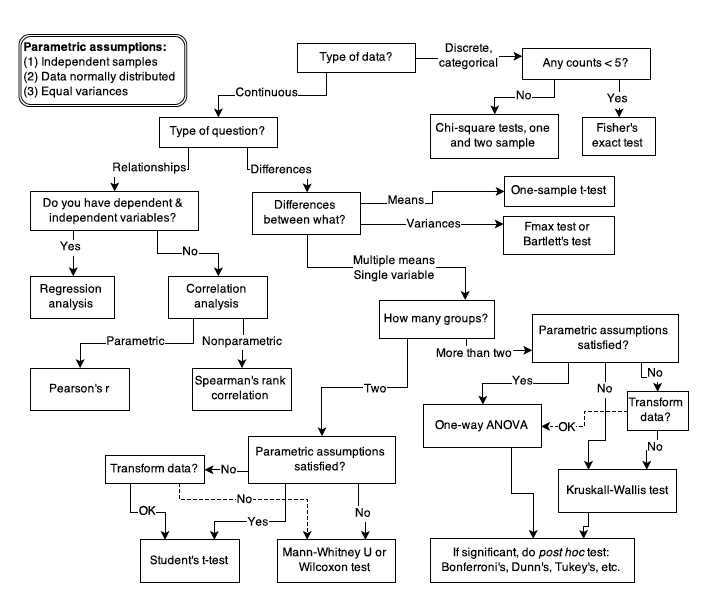
\includegraphics[width=9.89in]{./_images/fig1.1}

In addition, novel research often requires novel methods and the researchers may have to stray from the common tests to engineer their own golems.

\hypertarget{statistical-rethinking}{%
\section{Statistical Rethinking}\label{statistical-rethinking}}

\begin{quote}
A lot can go wrong with statistical inference, and this is one reason that beginners are
so anxious about it. When the goal is to choose a pre-made test from a flowchart, then the
anxiety can mount as one worries about choosing the ``correct'' test.
\end{quote}

More work is needed to ensure researchers understand all the moving parts of their golems and how to interpret their results.

\hypertarget{what-are-we-trying-to-do-with-the-golems}{%
\subsection{What are we trying to do with the golems?}\label{what-are-we-trying-to-do-with-the-golems}}

The popular belief is that we need to create models that use statistical means to test the null hypothesis.

Two reasons why deductive falsification doesn't work:

\begin{quote}
\begin{enumerate}
\def\labelenumi{\arabic{enumi}.}
\tightlist
\item
  Hypotheses are not models. The relations among hypothese and different kinds of models are complex. Many models correspond to the same hypothesis, and many hypotheses corresponf to asingle model. This makes strict falsification impossible.
\end{enumerate}
\end{quote}

All models are false, but some are useful.

Figure 1.2

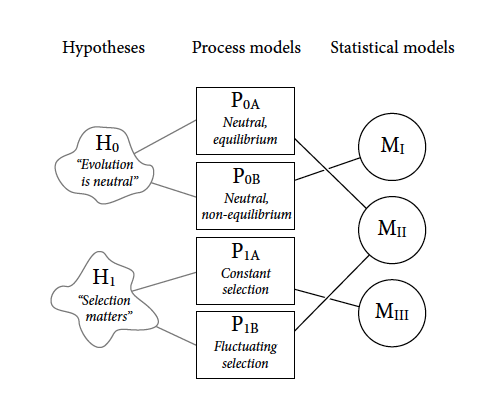
\includegraphics[width=6.86in]{./_images/fig1.2}

Two opposing hypothesis for evolutionary change:

H\textsubscript{0}: Neutral theory (random mutation and drift)

H\textsubscript{1}: Natural selection (fitness leads to observed change)

Process models for each hypothesis:

P\textsubscript{0a}: steady state in time (null)

P\textsubscript{0b}: fluctuations in population size through time

P\textsubscript{1a}: selection favours the same alleles through time

P\textsubscript{1b}: selection preference fluctuates through time (different alleles)

Statistical Models:

M\textsubscript{i}: unique to P\textsubscript{0b}

M\textsubscript{ii}: Power law in the data (frequency) shared expectation of \emph{P\textsubscript{0a} and P\textsubscript{1b}}

M\textsubscript{iii}: unique to P\textsubscript{1a}

\emph{Note that all process models contain time, solidifying directionality}

\begin{quote}
\begin{enumerate}
\def\labelenumi{\arabic{enumi}.}
\setcounter{enumi}{1}
\tightlist
\item
  Measurements matter. Even when we think the data falsify a model, another observer will debate our methods and measures. They don't trust the data. Sometime sthey are right.
\end{enumerate}
\end{quote}

\emph{The colour of swans}

Before Australia was discovered, all swans were white and no number of observations could prove this fact to be true.

H\textsubscript{0}: All swans are white

Australia had black swans, which instantly makes H\textsubscript{0} false.

Remember, observations are prone to error and hypotheses are quantitative rather than discrete.

\begin{quote}
``At the edges of scientific knowledge, the ability to measure a hypothetical phenomenon is often in question as much as the phenomenon itself.''
\end{quote}

\hypertarget{tools-for-golem-engineering}{%
\section{Tools for golem engineering}\label{tools-for-golem-engineering}}

\begin{quote}
You'll wreck Prague eventually, you just need to notice the destruction.
\end{quote}

We want our models to be able to design inquiry, extract information from data, and make predictions. To do this we will need:

\begin{enumerate}
\def\labelenumi{\arabic{enumi}.}
\tightlist
\item
  Bayesian data analysis
\item
  Model comparison
\item
  Multilevel Models
\item
  Graphical causal models
\end{enumerate}

\hypertarget{bayesian-data-analysis}{%
\subsection{Bayesian data analysis}\label{bayesian-data-analysis}}

Bayesian data analysis takes questions in the form of a model and produces logical probability distributions of the answer. This represents plausibility.

\hypertarget{model-comparison-and-predictions}{%
\subsection{Model comparison and predictions}\label{model-comparison-and-predictions}}

Model comparison is often thought of in terms of `which model will make the best predictions?' Two tools for this are Cross-validation and Information Criteria.

Complex models usually make worse predictions than simple ones due to \emph{overfitting}. The smarter the golem, the dumber its predictions. Fitting is easy; prediction is hard.

\hypertarget{multilevel-models}{%
\subsection{Multilevel models}\label{multilevel-models}}

\hypertarget{graphical-causal-models}{%
\subsection{Graphical causal models}\label{graphical-causal-models}}

\hypertarget{summary}{%
\section{Summary}\label{summary}}

\hypertarget{session-info}{%
\section*{Session Info}\label{session-info}}
\addcontentsline{toc}{section}{Session Info}

\begin{Shaded}
\begin{Highlighting}[]
\FunctionTok{sessionInfo}\NormalTok{()}
\end{Highlighting}
\end{Shaded}

\begin{verbatim}
## R version 4.1.1 (2021-08-10)
## Platform: x86_64-apple-darwin17.0 (64-bit)
## Running under: macOS Big Sur 10.16
## 
## Matrix products: default
## BLAS:   /Library/Frameworks/R.framework/Versions/4.1/Resources/lib/libRblas.0.dylib
## LAPACK: /Library/Frameworks/R.framework/Versions/4.1/Resources/lib/libRlapack.dylib
## 
## locale:
## [1] en_CA.UTF-8/en_CA.UTF-8/en_CA.UTF-8/C/en_CA.UTF-8/en_CA.UTF-8
## 
## attached base packages:
## [1] stats     graphics  grDevices utils     datasets  methods   base     
## 
## loaded via a namespace (and not attached):
##  [1] compiler_4.1.1  magrittr_2.0.1  fastmap_1.1.0   bookdown_0.26  
##  [5] htmltools_0.5.2 tools_4.1.1     rstudioapi_0.13 yaml_2.2.1     
##  [9] stringi_1.7.3   rmarkdown_2.14  knitr_1.33      stringr_1.4.0  
## [13] digest_0.6.27   xfun_0.30       rlang_0.4.11    png_0.1-7      
## [17] evaluate_0.14
\end{verbatim}

\hypertarget{small-worlds-and-large-worlds}{%
\chapter{Small worlds and large worlds}\label{small-worlds-and-large-worlds}}

Every model has two parts: small world and large world. \emph{The small world} is within the model itself and \emph{the large world} is the broader world we want the model to be applied to. In the small world, everything is defined and there isn't much room for pure surprises. The large world has more opportunities for unforeseen events and because the small world is an incomplete representation of the large world, mistakes are expected. The goal is to create small worlds (models) that approximate reality so that they perform well in the large world.

\hypertarget{the-garden-of-forking-data}{%
\section{The garden of forking data}\label{the-garden-of-forking-data}}

Bayesian inference is the counting and comparing of possibilities. At each point where a `decision' may split the path, bayesian inference evaluates each path and eliminates the paths that are not congruent with the data fed into the model.

\hypertarget{counting-possibilities}{%
\subsection{Counting possibilities}\label{counting-possibilities}}

\textbf{Marble Example}

There is a bag of four marbles of two colours (blue and white). This means that there could be 5 possibilities (conjectures); 4:0 white, 3:1 white, 2:2 split, 3:1 blue, and 4:0 blue.

A sequence of three marbles is pulled from the bag, one at a time, and returned to the bag (repeated sampling)\\
We get blue, white, blue.

Considering a 3:1 white scenario, on the first draw you could get a blue marble or three white marble draws\\

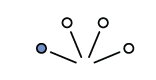
\includegraphics[width=2.17in]{./_images/fig2.1}

Expanding out one more draw (layer) we can expect the same possibilities because the first marble is replaced before the second draw\\

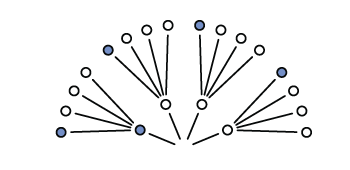
\includegraphics[width=4.86in]{./_images/fig2.2}

Expanding one more time gives us the final garden of 64 possibilities (4\textsuperscript{3}; 4 marbles with 3 draws)\\

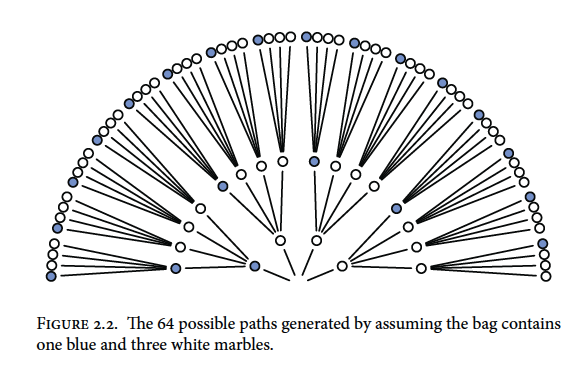
\includegraphics[width=8.06in]{./_images/fig2.3}

Now recall our draws were blue, white, blue so we can trim the paths that are not congruent with the draws\\

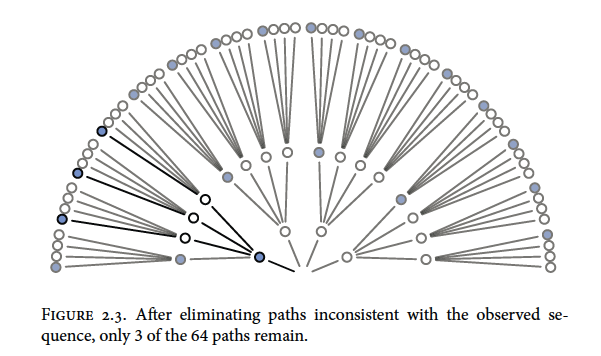
\includegraphics[width=8.35in]{./_images/fig2.4}

We can also trim other possibilities like all white marbles or all blue marbles because we drew both colours from the bag. Putting our 3:1 white, 2:2 split, and 3:1 blue possibilities together would look something like this\\

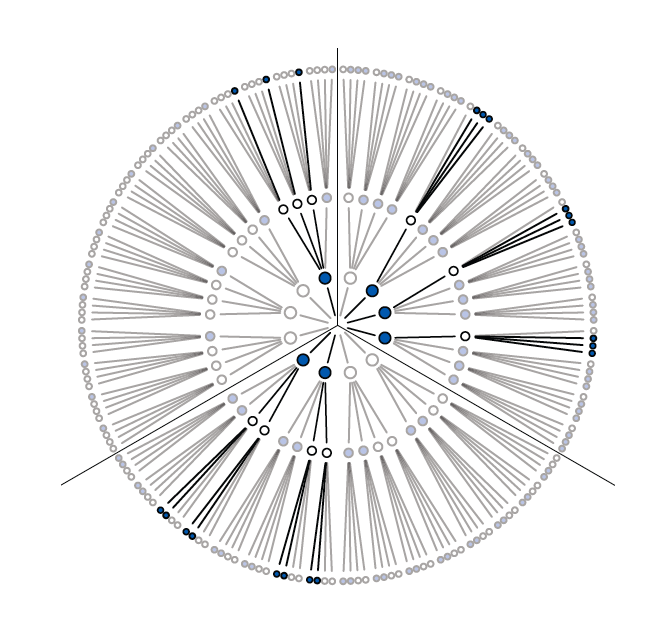
\includegraphics[width=9.28in]{./_images/fig2.5}

You can see that there are different numbers of unique paths to get our observed result\\
3:1 white has 3 paths\\
2:2 split has 8 paths\\
3:1 blue has 9 paths\\

We will call these counts our priors.

\hypertarget{combining-other-information}{%
\subsection{Combining other information}\label{combining-other-information}}

Suppose we make another marble draw and it is blue. We then count the ways each of our marble possibilities could create this new result\\

3:1 white has 1 paths\\
2:2 split has 2 paths\\
3:1 blue has 3 paths\\

Mutiplying by the prior counts gives us:\\

3:1 white has (3x1) 3 paths\\
2:2 split has (8x2) 16 paths\\
3:1 blue has (9x3) 27 paths\\

and suggests that our 3:1 blue possibility is more plausible with the new information.\\
\emph{Note that prior data and new data don't have to be of the same type}

\hypertarget{sampling-the-imaginary}{%
\chapter{Sampling the imaginary}\label{sampling-the-imaginary}}

\hypertarget{geocentric-models}{%
\chapter{Geocentric models}\label{geocentric-models}}

\hypertarget{the-many-variables-the-spurious-waffles}{%
\chapter{The many variables \& the spurious waffles}\label{the-many-variables-the-spurious-waffles}}

\hypertarget{the-haunted-dag-the-casual-terror}{%
\chapter{The haunted dag \& the casual terror}\label{the-haunted-dag-the-casual-terror}}

\hypertarget{equations}{%
\section{Equations}\label{equations}}

Here is an equation.

\begin{equation} 
  f\left(k\right) = \binom{n}{k} p^k\left(1-p\right)^{n-k}
  \label{eq:binom}
\end{equation}

You may refer to using \texttt{\textbackslash{}@ref(eq:binom)}, like see Equation \eqref{eq:binom}.

\hypertarget{theorems-and-proofs}{%
\section{Theorems and proofs}\label{theorems-and-proofs}}

Labeled theorems can be referenced in text using \texttt{\textbackslash{}@ref(thm:tri)}, for example, check out this smart theorem \ref{thm:tri}.

\begin{theorem}
\protect\hypertarget{thm:tri}{}\label{thm:tri}For a right triangle, if \(c\) denotes the \emph{length} of the hypotenuse
and \(a\) and \(b\) denote the lengths of the \textbf{other} two sides, we have
\[a^2 + b^2 = c^2\]
\end{theorem}

Read more here \url{https://bookdown.org/yihui/bookdown/markdown-extensions-by-bookdown.html}.

\hypertarget{callout-blocks}{%
\section{Callout blocks}\label{callout-blocks}}

The R Markdown Cookbook provides more help on how to use custom blocks to design your own callouts: \url{https://bookdown.org/yihui/rmarkdown-cookbook/custom-blocks.html}

\hypertarget{ulysses-compass}{%
\chapter{Ulysses' compass}\label{ulysses-compass}}

\hypertarget{publishing}{%
\section{Publishing}\label{publishing}}

HTML books can be published online, see: \url{https://bookdown.org/yihui/bookdown/publishing.html}

\hypertarget{pages}{%
\section{404 pages}\label{pages}}

By default, users will be directed to a 404 page if they try to access a webpage that cannot be found. If you'd like to customize your 404 page instead of using the default, you may add either a \texttt{\_404.Rmd} or \texttt{\_404.md} file to your project root and use code and/or Markdown syntax.

\hypertarget{metadata-for-sharing}{%
\section{Metadata for sharing}\label{metadata-for-sharing}}

Bookdown HTML books will provide HTML metadata for social sharing on platforms like Twitter, Facebook, and LinkedIn, using information you provide in the \texttt{index.Rmd} YAML. To setup, set the \texttt{url} for your book and the path to your \texttt{cover-image} file. Your book's \texttt{title} and \texttt{description} are also used.

This \texttt{gitbook} uses the same social sharing data across all chapters in your book- all links shared will look the same.

Specify your book's source repository on GitHub using the \texttt{edit} key under the configuration options in the \texttt{\_output.yml} file, which allows users to suggest an edit by linking to a chapter's source file.

Read more about the features of this output format here:

\url{https://pkgs.rstudio.com/bookdown/reference/gitbook.html}

Or use:

\begin{Shaded}
\begin{Highlighting}[]
\NormalTok{?bookdown}\SpecialCharTok{::}\NormalTok{gitbook}
\end{Highlighting}
\end{Shaded}

\hypertarget{conditional-manatees}{%
\chapter{Conditional manatees}\label{conditional-manatees}}

\hypertarget{markov-chain-monte-carlo}{%
\chapter{Markov chain monte carlo}\label{markov-chain-monte-carlo}}

\hypertarget{big-entropy-and-the-generalized-linear-model}{%
\chapter{Big entropy and the generalized linear model}\label{big-entropy-and-the-generalized-linear-model}}

\hypertarget{god-spiked-the-integers}{%
\chapter{God spiked the integers}\label{god-spiked-the-integers}}

\hypertarget{monsters-and-mixtures}{%
\chapter{Monsters and mixtures}\label{monsters-and-mixtures}}

\hypertarget{models-with-memory}{%
\chapter{Models with memory}\label{models-with-memory}}

\hypertarget{adventures-in-covariance}{%
\chapter{Adventures in covariance}\label{adventures-in-covariance}}

\hypertarget{missing-data-and-other-opportunities}{%
\chapter{Missing data and other opportunities}\label{missing-data-and-other-opportunities}}

\hypertarget{generalized-linear-madness}{%
\chapter{Generalized linear madness}\label{generalized-linear-madness}}

\hypertarget{horoscopes}{%
\chapter{Horoscopes}\label{horoscopes}}

  \bibliography{book.bib,packages.bib}

\end{document}
